
\documentclass[11p]{article}
% Packages
\usepackage{amsmath}
\usepackage{graphicx}
\usepackage[swedish]{babel}
\usepackage[
    backend=biber,
    style=authoryear-ibid,
    sorting=ynt
]{biblatex}
\usepackage[utf8]{inputenc}
\usepackage[T1]{fontenc}
%Källor
\addbibresource{mall.bib}
\graphicspath{ {./images/} }

\title{Kärnkraft \\ \small Fysik 1}
\author{Noel Johansson }
\date{\today}

\begin{document}

    \begin{titlepage}
        \begin{center}
            \vspace*{1cm}

            \Huge
            \textbf{Kärnkraft}

            \vspace{0.5cm}
            \LARGE


            \vspace{1.5cm}

            \textbf{Noel Johansson}

            \vfill

            Ett PM om energiförsörjning \\
            Fysik 1

            \vspace{0.8cm}

            
\includegraphics[width=0.4\textwidth]{../images/NTI Gymnasiet_Symbol_print_svart.png}

            \Large
            Teknikprogrammet\\
            NTI Gymnasiet\\
            Umeå\\
            \today

        \end{center}
    \end{titlepage}
% Om arbetet är långt har det en innehållsförteckning, annars kan den utelämnas
    \tableofcontents
    \newpage



    \section{Inledning}
    Kärnkraftverk är en av de mest kontroversiella energikällor som finns men finns det verkligen någon anledning till detta?
    \subsection{frågeställningar}
    \begin{enumerate}
        \item Hur fungerar ett kärnkraftverk?
        \item Vad för miljöpåverkan har kärnkraftverk på både lokal och global skala?
        \item Hur påverkar kärnkraft och kärnkraftverken samhället på både lokal och global skala?
    \end{enumerate}

    \section{Resultat}

    \subsection{Kärnkraft, så fungerar det}
    För att få energi från Uranium krävs fission alltså att klyva atomen itu.
    När man skall klyva en atom så skickas en neutron in i atomkärnan på Uran och detta gör så att atomkärnan blir instabil.
    När atomkärnan blir instabil så splittras atomen och i denna splitring så skapas energi.
    Atomens splitring gör så att uranet delas på två delar men det skickas även ut två styckna neutroner och i ett kärnkraftverk så använder man neutronerna som skickas ut för att klyva andra uranatomer.
    Att neutroner som är resultatet av en klyvning sedan klyver en annan atom kallas för kedjereaktion.

    I ett kärnkraftverk så har man en stor mängd uran och sedan så börjar man klyva en atom och sedan så använder man sig av kedjereaktioner för att fortsätta processen.
    Energin som kommer från fissionen värmer upp vatten och värmeenergin från vattnet omvandlas till rörelse energi i turbiner som alltså börjar snurra av energin.
    Turbinernas rotation genererar elektricitet.
    \parencite{Wikipedia}
    \parencite{TekniskaMuseet}


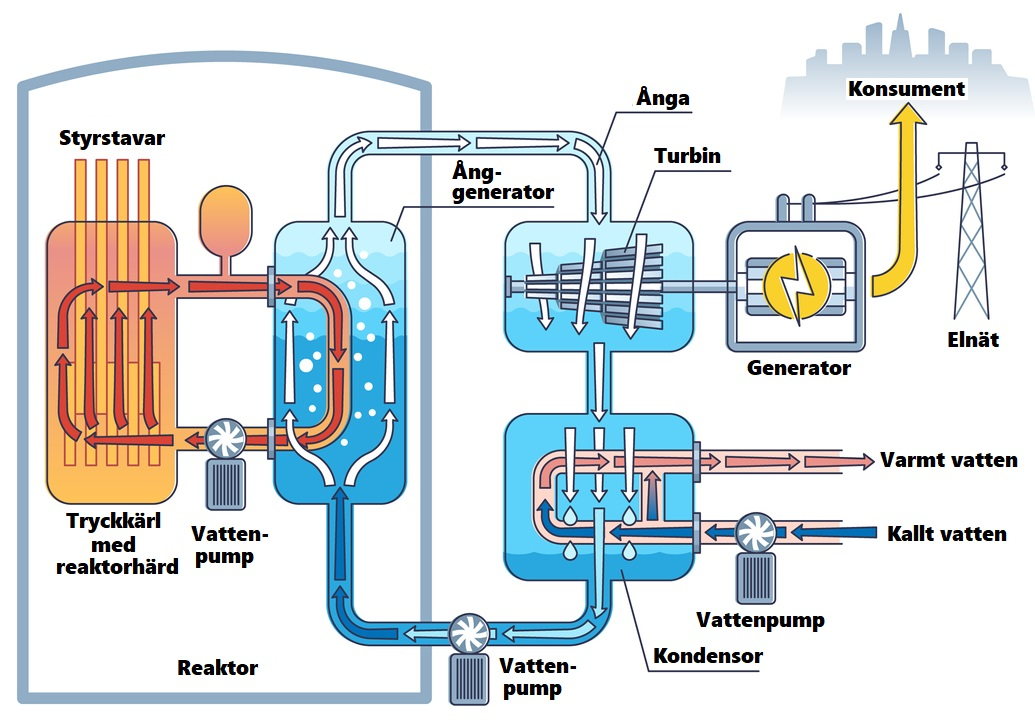
\includegraphics[width=0.4\textwidth]{../images/karnkraftverk-2.jpg}


    \subsection{Miljökonsekvenser av kärnkraft}
    Kärnkraftverk genererar relativt låg mängd av koldioxid jämfört med andra alternativ.
    \textcite{Vattenfall} har gått ut med att alla sveriges kärnkraftverk genomsnittligt genererar 2,5 gram koldioxid per kilowattimme.
    Kärnkraftverk är dock väldigt farliga för väldigt små misstag kan leda till stora konsekvenser.
    Eftersom uran är radioaktivt så måste det hanteras väldigt noggrant och om det skulle ske en olycka på ett kärnkraftverk kan strålning sprida sig och göra stora områden helt livsodudliga.
    Efter en atom klyvits så blir det avfall från uranet och detta avfall är också radioaktivt.
    Detta avfall behövs förvaras på säkra ställen så att de inte kan göra någon skada.
\parencite{Vattenfall2}
    \subsection{Samhällets syn på kärnkraft}
    Kärnkraftverk är ett väldigt effektivt sätt att generera energi men på grund av hur rädda folk är av radioaktivitet så hindras många kärnkraftverk från att bli byggda.
    2011 så drabbades Fukushima i Japan av en stor kärnkraftsolycka i samband med en jordbävning och på grund av den så är Fukushima än i dag obeboligt.
    Olyckan i Fukushima påminde folk runt omkring världen att kärnkraft är farligt och detta har gjort så att många personer är rädda för kärnkraft.



    \section{Slutsatser}
    Kärnkraft är potentiellt extremt farligt och dödligt men under bra säkerhet så är det den mest effektiva energikällan vi är medvetna om just nu.
    Att satsa på kärnkraft är en stor risk men jag tycker det är värt chansen för det vi har att vinna på det är väldigt stort.
    Det krävs många säkerhetsåtgärder för att producera kärnkraft säkert men jag tror att kärnkraft är framtiden och att alla länder borde jobba för att få fram säkra kärnkraftverk.

% Mer saker som du kan ha nytta av.








    \printbibliography

\end{document}